\section{Introduction}

FOSS\footnote{Free and Open-Source Software \cite{stallmann2021copyleft}} is
generally defined as software the user can \textit{``[...] run, copy,
distribute, study, change and improve [...]''} \cite{fsf2024whycopylef}. This
requires the source to be available and enables the dependence of other
software on subsets or the entirety of the code. On the other hand, source
available or OSS\footnote{Open-Source Software} are distinct from FOSS
software. Some licenses do not require the resulting product to be licensed
under the same license as its dependencies, such as the MIT
license\footnote{Requires the license to be present in \textit{``all copies or
substantial portions of the Software''} \cite{osorg2024mit}}. It therefore
differs from the GPL\footnote{Requires all copies of the software to be
licensed as GPL \cite{osorg2024gpl}} and software licensed with the MIT-Licence
can therefore not be referred to as free open-source software, but rather as
open-source software. \newline Most OSS-projects accept contributions from
individuals and enterprises. This is wanted and required to support the
actuality of said software. Most OSS projects accept changes matching their
pre-defined contribution guidelines and credit the contributor for their
addition. These contributors often use the software they are contributing to
and therefore make changes they care for, such as adding drivers for new
devices to the Linux kernel \cite{linuxUnknownDevicedrivers}. \newline However,
other independent OSS contributors are abusing the contribution system by
exploiting the trust the unpaid maintainers have in the quality of the
submitted changes. Specifically, this refers to manipulating maintainers and
inserting oneself into the group of by applying pressure on said group. As was
the case with \texttt{liblzma} or the \texttt{xz-utils} OSS library.

\subsection{Dependence on FOSS and OSS}

Open source software is often divided into reusable components, such as
libraries or toolkits implementing a specific feature, and built upon by other
software. The goal is to use tried and tested components in the creation of new
OSS, thus building on field tested and established software found in the OSS
community.

Not only does OSS depend on other libraries from the OSS ecosystem. Proprietary
software also makes use of said OSS components, while being forced to adhere to
their terms, as declared in their respective licenses \cite{libcurl2024usage}. 


\begin{figure}[H]
    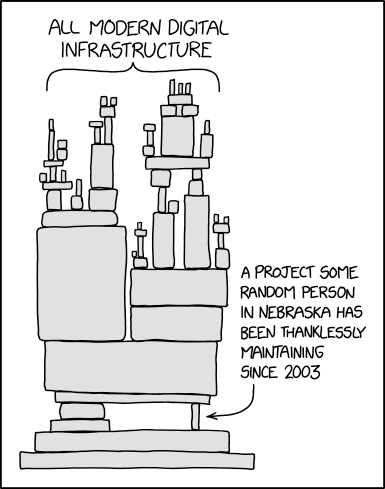
\includegraphics[scale=0.5]{assets/dependency.png}
    \caption{Dependency \cite{xkcdUnknownDependency}}
    \label{img:dependency}
\end{figure}

Commonly used examples for said libraries are \texttt{libcurl}, which provides
multi protocol file transfers \cite{libcurl2024overview}, \texttt{raylib} which
is a library for video games programming \cite{raylib2024landing} and the
\texttt{sqlite} library, that implements a in process database
\cite{sqlite2024landing}. These library examples are so widely used, a
vulnerability in them would impact the security of the whole software space.

\subsection{Supply Chain Security}

Supply chain security is referring to the fact of ensuring the dependencies of
a given software are to be considered secure and making sure this property can
be accessed to be true. This can be achieved by keeping the development
tool-chain used for creating said software up to date, thus patching and
removing found vulnerabilities \cite{ccc2024supplychainsec}. Other ways of
establishing the security of a dependency is to manually evaluate the source
code of the given dependency.

However most largely used open source software is thoroughly tested and
famously so. \texttt{sqlite} prides itself as being the \textit{''most used and
deployed database engine``} \cite{sqlite2022mostdeployed} and \textit{''[...]
the project has 590 times as much test code and test scripts [as lines of
source code]``} \cite{sqlite2022testing}. 

Considering the large amount of memory safety errors\footnote{70\% according to
\cite{googleUnknownMemorySafety}}, often caused by invalid or maliciously
crafted input, projects entirely focussed around detecting said
vulnerabilities, such as \texttt{OSS-Fuzz} \cite{google2024fuzzing}, saw their
inception.

\subsection{xz-utils and liblzma}

\texttt{xz-utils} refers to a c implementation of the \texttt{xz}
compression algorithm and format. It is written to comply with the C99
standard and consists of several components. One of these components is, as
previously introduced, a library providing an API for compression and
decompression \cite{tukaani2024xz}.

\cite{ccc2024backdoor}
